\chapter{腹侧前额叶皮层:基于视听内容生成目标}
这本书提出了关于灵长类动物前额叶皮层基本功能的方案。
腹侧 PF 皮层根据视觉和听觉线索生成目标,我们称之为标志,它的连接解释了为什么只有它才能做到这一点。腹侧 PF 皮层与颞下皮层的视觉区和颞上皮层的听觉区以及其他PF区有联系。它与颞叶皮层的连接提供了视觉和听觉信号,从而建立了当前的行为环境。眼眶 PF 皮层提供了选择和结果之间的联系,有时可以在单个事件的基础上学习(第4章)。在许多任务中,腹侧 PF 皮层根据具体物体和地点生成目标。然而,在涉及抽象规则和策略的任务中,腹侧PF皮层可以生成一组或几类目标以供选择或避免。鉴于腹侧PF皮层在类人猿灵长类动物中进化(第2章),我们认为它在使用视觉标志和声音信息方面具有优势,可以指导近距离和远距离的觅食选择。
\section{介绍}
\par
正如第 2 章所指出的,人们经常将灵长类动物描述为“视觉动物”。原因是中央凹在早期的单鼻科动物中进化,而三色视觉在类人猿中进化。 这些进步使这些动物及其后代能够辨别位置、颜色、形状、视觉纹理、光泽度和半透明度的微小差异。本章回顾了类人猿使用这些视觉特征来提供觅食机会线索的证据,我们称之为标志。正如第2章所解释的那样,我们所说的符号是指用作提示但不一定对应于整个对象的非空间景象和声音。
\par
进化已经设计出许多方法来获得觅食优势。一些哺乳动物通过精心制作身体部位来开发资源,从而利用了它们的生态位。大象的长鼻子使它们能够以其他哺乳动物无法做到的方式觅食。长颈鹿的长脖子同样提供了独特的觅食机会。我们认为,类人猿反而精心设计了某些大脑结构,包括腹侧PF皮层。
\begin{figure}
	\centering
	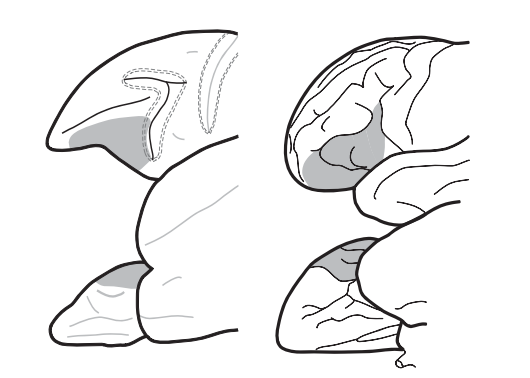
\includegraphics[width=0.7\linewidth]{image_pfc/Fig_7_1}
	\caption{猕猴(左)和人类(右)的腹侧PF皮层。格式如图1.2所示。}
	\label{fig:fig}
\end{figure}
\par
前一章解释了背侧PF皮层生成适合当前上下文的目标,如最近事件指定的,尤其是视觉事件。它解释了视觉线索的顺序、位置和时间的重要性,以及其他特征,强调与后顶叶皮层的联系。腹侧PF皮层与下颞叶皮层和上颞叶皮层相连。因此,可见或可听的标志也指定了当前的上下文,类人猿可以单独使用或结合由顺序、位置和时间确定的上下文使用。
\section{区域}
\par
在猕猴中,腹侧PF皮层包括主沟腹侧半球的外侧凸起(图 7.1)。在人类中,同源区域位于额下回。在两者中,腹侧PF皮层围绕半球的外侧末端延伸至外侧眶沟。术语12/47由Petrides和Pandya设计,反映了他们认为人类的47区与猴子的12区同源的观点(Petrides\&Pandya 2002b)。
\par
就细胞结构区域而言,腹侧PF皮层包括猕猴的45区和12/47区(见图 1.2)。在人类中,腹侧PF皮层包括区域45和47。
\section{连接}
\begin{figure}
	\centering
	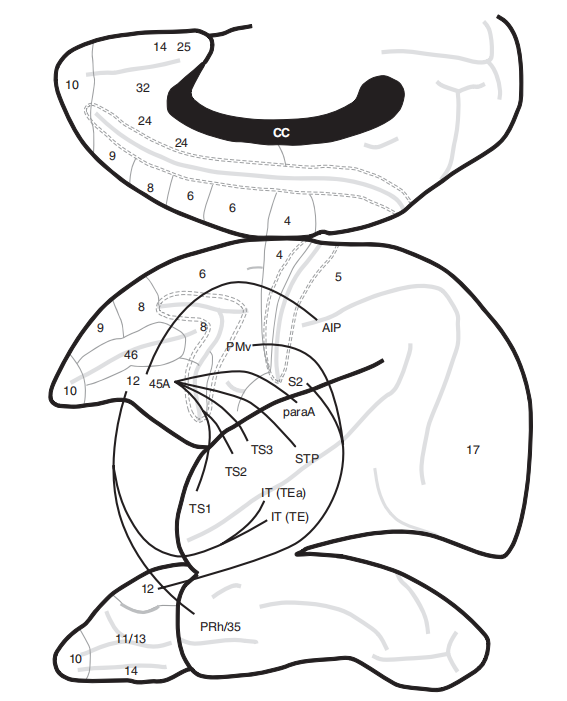
\includegraphics[width=0.7\linewidth]{image_pfc/Fig_7_2}
	\caption{腹侧PF皮层的选定连接。图1.4和1.5给出了脑沟和区域的名称。线连接一些与腹侧PF皮层具有直接轴突连接的区域,除非另有说明,否则假定它们是相互的。}
	\label{fig:fig}
\end{figure}
图7.2显示了腹侧PF皮质的皮质皮质连接。有几个特点很突出:
\begin{enumerate}
\item 如前所述,腹侧PF皮层与颞叶紧密相连。腹侧PF皮层与下颞叶皮层相互联系。格式如图1.2所示。连接197(Ungerleider et al. 1989;Webster et al. 1994)和颞上皮层(Seltzer et al. 1996;Petrides \&Pandya 2002b)。它也与鼻周皮质有联系(Suzuki \& Amaral 1994 ; Saleem et al. 2008),尽管没有那么多。 
\par
这些联系有两个含义。首先,腹侧PF接收有关指定行为环境的信号或标志的信息。下颞叶皮层在辨别颜色、形状和视觉纹理方面起着至关重要的作用(Huxlin et al. 2000) 。颞上皮层参与声音识别(Tian et al. 2001)和声音序列(Micheyl et al. 2005),包括其他动物的叫声(Rauschecker et al. 1995)。 
\par
其次,到达腹侧PF皮层的信息来自高级和中级视觉区域,而不是来自低级视觉区域。通过高阶视觉,我们指的是一个物体特征的广泛结合,这是鼻周皮质所代表的(Murray et al. 2007)。相比之下,下颞区,如TE区,构建了介于整个对象的表示及其基本特征之间的中级连词(Murray et al. 2007)。最尾部的视觉区域构建低阶连词,一些代表基本特征,但这些区域不投射到腹侧PF皮层(Webster et al,1994)。在这方面,腹侧PF皮层的连接与尾侧PF皮层的连接不同(第5章)。
\item 腹侧PF皮层还与第二体感区 (S2) 附近的一组复杂区域相互连接(Petrides \& Pandya 2002b)。因此,腹侧PF皮层接收来自视觉、听觉和躯体感觉皮层的多模式输入。S2内部和周围的皮层有助于物体的触觉辨别(Mishkin 1979),而鼻周皮层对于通过视觉或触觉识别物体至关重要(Goulet \& Murray 2001;Murray et al. 2007)。
\item 腹侧PF皮层接收来自下顶叶区PG的输入(Petrides \& Pandya 2002b)。此连接可能会提供有关对象位置的信息。腹侧PF皮层还接收来自后顶叶区域AIP的输入,这似乎在猴子拾起物体时使用视觉来校准抓握方面发挥作用(Fogassi et al,2001)。
\item 腹侧 PF 皮层(区域 12/47)与腹侧前运动皮层的延髓部分有很强的联系。 最近的一份报告称这部分运动前皮层区域为 F5a(Gerbella et al,2011),第2章提到该区域似乎控制手和嘴的运动。 
\item 腹侧PF皮层也与杏仁核有关。一些神经解剖学迷雾将这些描述为广泛的(Amaral \& Price 1984 ;Stefanacci \& Amaral 2002),但其他人认为它们稀疏(Carmichael \& Price 1995a;Price \& Drevets 2010)。无论如何,与杏仁核的连接可能会提供更新的估值,如第3章和第4章所解释的那样,直接连接到腹侧 PF皮层或通过眼眶PF皮层间接连接。包括下颞叶皮层(Horel et al. 1975)或杏仁核(Horel et al. 1975;Aggleton \& Passingham 1981)在内的损伤会影响物体看起来有吸引力还是令人厌恶,并且两者都与腹侧PF皮层有关。
\end{enumerate}
\subsection{总结}
腹侧 PF 皮层从下颞叶皮层和上颞叶皮层接收有关视觉和听觉信号的信息,并且它可以将当前行为背景的这些方面与来自杏仁核或眼眶 PF 皮层的结果信息整合(Barbas \& Pandya 1989),或两者皆有。

\section{视觉和听觉条件任务}
\par
鉴于其与颞叶的联系,腹侧 PF 皮层可以使用有关视觉和听觉环境的信息来生成目标。 实验室实验可以通过使用条件任务来测试这种能力。 这些任务涉及视觉和听觉条件任务 199 上下文和适当目标之间的任意映射。因此,例如,猴子可能会在提示 A 出现后学习它们应该选择对象 1,但在提示 B 出现后它们应该选择对象 2。
\par
当视觉上下文映射到视觉目标时,该任务称为条件视觉-视觉学习或配对联想学习。 当视觉上下文映射到空间上下文或直接映射到动作时,它通常称为条件视觉空间学习、条件视觉运动学习或条件运动学习。我们在整本书中使用条件视觉运动学习。
\par
腹侧 PF 皮层至少通过钩突束接收一些关于视觉世界的信息。 该纤维通路连接下颞叶皮层和腹侧 PF 皮层中的细胞 (Ungerleider et al. 1989)。 切断这条通路会导致 monkeys 比正常情况下更慢地学习条件视觉-视觉关联 (Eacott \& Gaffan 1992 ; Gutnikov et al. 1997)。还可以教猴子一项有条件的听觉-视觉任务。 Gaffan 和 Harrison (1991) 教猴子在六种不同的视觉刺激中进行选择,每种视觉刺激由六种音调中的一种指示。 然后他们将 PF 皮层与颞上皮层断开,通过在一个半球制造 PF 皮层损伤和在另一个半球制造上颞叶皮层损伤。 他们切断了两个大脑半球之间的联系,以完成断开连接。 之后,猴子的表现无法超过偶然水平。
\par
一旦猴子学会了这类任务,就可以在颞叶中发现反映所学关联的细胞活动。 例如,Miyashita和他的同事向猴子展示了一系列复杂的颜色和形状刺激,并教它们在成对的这些刺激之间进行任意关联(Sakai 和 Miyashita 1991 年;Naya et al. 1996 年)。 在动物学会配对后,颞下皮层的细胞编码这些关联,Miyashita 和他的同事称这些配对编码细胞。 成对编码细胞显着出现在鼻周皮质和头端颞下
皮质和较少发生在更尾部的下颞区 (Naya et al. 1996, 2001)。
\par
为了表明这些特性来自学习,Messinger 等人。 (2001) 研究了 monkeys 学习条件视觉-视觉关联时鼻周皮质和颞下皮质细胞活动的变化。 他们发现在学习的初始阶段形成了配对编码属性关系。 不幸的是,他们的猴子在 Messinger 等人的有限时间内只了解了一点有关协会的信息。 可以研究每个细胞的活动。
\par
宫下等人(2004) 提供的证据表明这些关联的检索取决于 PF 皮层。 实验者切除了胼胝体的尾部,同时保留了左右 PF 皮层之间的连合连接(Tomita et al. 1999 年)。 然而,向右颞叶呈现提示会为其在左颞叶的目标刺激生成配对编码活动。 这些结果表明,有关线索刺激的信息从右颞叶到右 PF 皮层,然后到左 PF 皮层,最后回到左颞叶 (Hasegawa et al. 1998 ; Tomita et al. 1999)。
\par
如果是这样,那么 PF 皮层中的细胞活动应该编码两张图片之间的关联。 雷纳等人。 (1999) 教猴子两项使用相同图片作为刺激的任务:一项涉及视觉-视觉映射,另一项涉及匹配样本规则。 延迟期早期的活动通常编码提示,但延迟期后期的活动通常编码目标。 这些结果证实了前瞻性编码在 PF 皮质中的存在,并且至少将该功能的一部分定位于腹侧 PF 皮层。
\par
我们说这些结果证实了前瞻性编码,因为 Gaffan (1977) 已经在行为上表明,在有条件的视觉运动任务中,猴子会在延迟期间对目标进行编码。 他操纵了指令提示颜色和目标位置的相似性,并推断如果猴子在延迟期间回顾性地编码指令提示,它们应该混淆相似的提示,并且它们会通过错误的选择反映这种混淆。 相比之下,如果猴子对当前目标进行前瞻性编码,它们会将附近的目标位置相互混淆。 研究结果支持前瞻性编码。 因此,在延迟期间,猴子主要在记忆中持有目标,而不是线索,以及 Rainer 等人的结果。 显示腹侧 PF 皮层中的神经元前瞻性地编码目标。

\par
腹侧 PF 皮层有助于学习线索和目标之间的关联,包括听觉或视觉线索何时指导选择。在提示和目标实现之间的延迟期间,猴子前瞻性地编码目标,腹侧 PF 皮层中的细胞有助于这种前瞻性编码。

\section{视觉空间和视觉运动协会}
\par
除了对象和图片之外,动作或位置也可以作为条件任务中的目标。 因此,任意视觉线索可以与手部运动(Bussey et al. 2001 年)或眼球运动(Asaad et al. 1998 年)相关联。 这些映射可以被视为条件视觉空间关联或条件视觉运动关联。 具有腹侧和眼眶 PF 病变联合病变的猴子在这种学习关联方面有严重的损害(Bussey et al. 2001 年)。 仅腹侧 PF 皮层的失活会产生类似的效果 (Wang et al. 2000)。
\par
Boussaoud 和 Wise (1993) 从腹侧 PF 皮层的尾部记录了猴子执行各种版本的条件视觉运动任务。 在不同的试验中,相同的刺激可以提示不同的手部动作,不同的刺激可以提示相同的动作。 只有 百分之16-18的PF皮层细胞编码运动而不是提示的特征。相比之下,在背侧前运动皮层中,百分之51-64 的细胞对运动进行编码。 这种差异表明视觉标志在腹侧 PF 皮层功能中的重要性。
\par
如果腹侧 PF 皮层根据学习到的提示上下文生成目标,那么人们可能会期望学习过程中的激活发生变化。 所以托尼等人。 (2001) 教人类受试者移动不同的手指以响应不同的视觉信号。 在他们的实验中,受试者必须在扫描过程中通过反复试验来学习任意映射,其中在每次试验结束时给出反馈。 在控制条件下,箭头指向适当的手指,受试者只需按照指示执行,无需学习任何任意映射。 该分析寻找随着时间的推移激活的增加与控制条件相比学习。 这种增加发生在下颞叶皮层和腹侧和背侧 PF 皮层。
\par
然而,这个实验有两个因素区分了实验和控制条件:学习和使用任意线索。 所以 Boettiger 和 D’Esposito( 2005 ) 比较了受试者通过以下方式学习提示动作关联的情况在控制条件下进行试验和错误,其中受试者已经学会了关联扫描前。 因此,在他们的实验中,这两个条件的不同之处仅在于学习发生在实验条件下,而不是控制条件下。 正如 Toni 等人的实验一样。 ( 2001 ),学习相关的激活变化发生在腹侧和背侧 PF 皮层。
\par
与学习相关的激活增加可能反映了将 ping 线索映射到行动的具体情况,但它们可能只是反映了对结果的关注增加。这个问题可以通过从猴子的细胞中记录来解决。 阿萨德等人。 ( 1998 ) 任教猴子必须将任意提示与向左或向右的扫视联系起来。 在背侧和腹侧 PF 皮层的任务相关细胞中,百分之44的编码了特定提示和相关的扫视。 此外,随着学习的进展,活动响应编码在延迟期间逐渐提早发生。 这活动的变化似乎不太可能反映出对结果的关注。 调查人员可以比较与相同相关联的其他提示和眼跳组合结果,从而排除注意力和结果编码效应,至少对于这些细胞而言。
\par
在这些实验中,随着调查人员反复改变两个刺激和两个目标之间的映射,猴子学会了新的提示-动作关联。 然而,克罗默等。 ( 2011a ) 使用新颖的刺激。 猴子学得很快,与学习相关的活动发生在PF与皮层并联表现的变化。 它发生在审判的早期,就像 Asaad 等人早期的实验一样。 (1998)。
\subsection{总结}
腹侧PF皮层在学习视觉线索之间的新关联方面起着关键作用和空间目标或行动。证据表明 PF之间存在密切的对应关系皮层活动和学习根据线索上下文和损伤产生目标包括腹侧 PF皮层严重扰乱了新提示-目标映射的学习。第 8 章重新讨论了这个主题。
\section{样本匹配任务}
\par
条件任务涉及线索和目标之间的任意关联。 在这方面,这些任务不同于匹配样本任务,后者的目标必须与样本匹配。匹配任务为线索和目标之间的关系强加了一个身份规则,如反对猴子必须在有条件的任务中学习的武断规则。 然而,monkeys 仍然需要学习选择与样本匹配的对象或图片,并且在那感觉他们需要使用当前提示作为选择目标的背景。
\par
 根据这个想法,证据表明腹侧 PF 皮层起着关键作用在学习匹配样本任务中。 拉什沃思等。 (1997a) 测试了患有腹侧 PF 病变的猴子同时匹配颜色。 此任务使用与延迟匹配样本任务。 在任务的同步版本中,样本当猴子做出选择时仍然可见;在无延迟版本(也称为零秒延迟版本)中,样本在选择刺激出现的同时消失。
\par
在 Rushworth 等人的实验中,去除腹侧 PF皮层会导致重新学习同时匹配样本任务的显着障碍(图 7.3)。同样的结果发生在腹侧和眼眶 PF 皮层联合损伤后(Bussey et al. 2001)。并且,对于无延迟匹配,腹侧和眼眶的断开来自下颞叶皮层的 PF 皮层造成损伤(Bussey et al. 2002 )。
\par
我们可以为这些结果设计三个帐户:
\begin{enumerate}
\item 猴子可能有知觉障碍。 然而,Bussey 等人。 (2001)对他们的猴子进行了视觉辨别测试,他们正常地学习了。
\begin{figure}
	\centering
	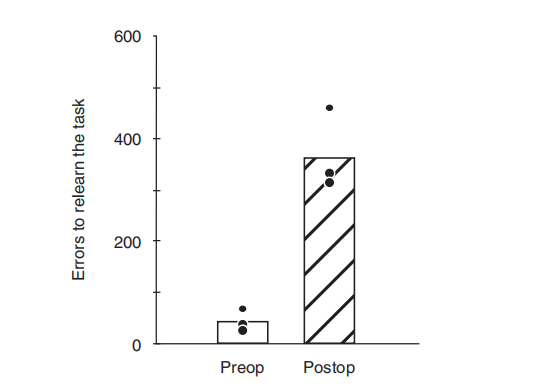
\includegraphics[width=0.6\linewidth]{image_pfc/Fig_7_3}
	\caption{腹侧 PF 皮层损伤对同步样本匹配任务的影响匹配。在同时匹配中,样本在选择时保持可见。一组猴子的术前 (preop) 和术后 (postop)表现,在中断(白色条)和损伤后重新学习任务所需的错误数(阴影线)绘制在纵坐标上。 实心圆圈表示个人的表现
	猴子。 转载自 Rushworth MF、Nixon PD、Eacott MJ、Passingham RE腹侧前额叶皮层对工作记忆不是必需的。 神经科学杂志 17:4829–38,© 神经科学协会,1997,经许可。}
	\label{fig:fig}
\end{figure}
\begin{figure}
	\centering
	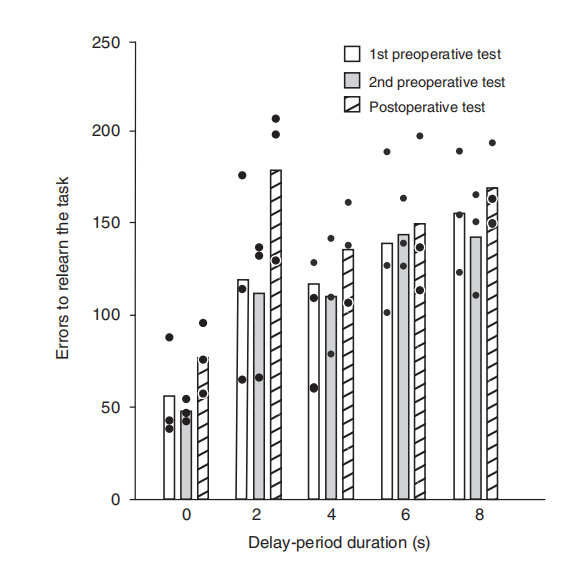
\includegraphics[width=0.6\linewidth]{image_pfc/Fig_7_4}
	\caption{腹侧 PF 皮层损伤对延迟匹配样本任务的影响,作为函数的延迟间隔。 两个术前测试的格式如图 7.3 所示(白色和灰色条)和损伤后的一项测试(阴影线)。 转载自 Rushworth MF、Nixon PD、Eacott MJ,Passingham RE。 腹侧前额叶皮层对工作记忆不是必需的。 杂志神经科学 17:4829–38, © Society for Neuroscience, 1997,经许可。}
	\label{fig:fig}
\end{figure}
\item 猴子可能会尝试记住样本,即使它们不需要,因此,结果可能反映了工作记忆的损害。 然而,这种解释无法解释 Rushworth 等人的研究结果。 他们的猴子重新学习了同步匹配任务,因此 Rushworth 等人。 可以在样本和样本之间以不同的延迟时间重新测试受损的猴子选择刺激。 与手术前相比,他们在延迟匹配方面没有犯更多错误(图 7.4)。 科瓦尔斯卡等。 ( 1991 ) 同样发现,一旦有腹侧 PF 的猴子病变重新学习了任务规则,它们在延迟的非匹配采样任务上正常执行,延迟时间长。
\par
 我们知道延迟期活动发生在腹侧和眼眶 PF 皮层(Rosenkilde et al. 1981 ; Hoshi et al. 2000) 并且延迟期激活发生当人类受试者执行延迟匹配样本任务时(Rama \& 考特尼 2005 年; 舍恩等人。 2008 年)。 我们知道电刺激延迟期间的眼眶 PF 皮层会导致 mon keys 中这些任务的损伤 (Sobotka et al. 2005)。 所以我们不否认一些活动的存在用回顾性工作记忆来解释。 而且我们不否认破坏这些区域的神经活动会导致这些任务的缺陷。 然而,Rushworth 等人的结果。 证明同时发生减值样本匹配任务不能归因于工作记忆问题:他们受伤的猴子在相当长的延迟后表现正常重新学习了任务规则。
\item 拒绝前两个说法留下了第三种可能的解释。 损伤后,猴子不再知道任务规则,因此它们必须重新学习。 在里面匹配样本任务,猴子必须使用身份规则:选择匹配样本的对象匹配样本。 在本章的后面,我们引用了 PF 中细胞活动的证据反映当前任务规则的皮层 (Wallis et al. 2001)。 造成的损害通过电刺激 (Sobotka et al. 2005 ) 可能是由于未能保留规则。
\end{enumerate}
\subsection{总结}
\par 
本章至此,腹侧 PF 皮层在视觉或听觉线索到目标或行动的任意映射中起着关键作用。 但是它的功能扩展了超越这样的协会。 在匹配样本任务中,提示和目标不是任意的。 当猴子在损伤前学习匹配规则时腹侧 PF 皮层,它们显示出在损伤后应用该规则的障碍。然而,腹侧 PF 损伤的猴子可以重新学习该规则,此后它们表现出正常的工作记忆能力。 因此,它们对样本匹配任务的损害发生了,因为受损的猴子在受损后不再立即知道规则。
\section{分类}
\par
如果腹侧 PF 皮层有助于通过颜色或形状进行匹配,并且还有助于学习关联不同的图片,那么人们可能会期望它也会在学习刺激类别方面发挥作用。 弗里德曼等人。 ( 2001 , 2002 ) 使用延迟匹配样本任务教猴子区分猫和狗的图画。 他们制作了一系列经过分级的变形图画,猴子学会了“猫”类别和“狗”类别之间的界限(图 7.5)。 可以在延迟期间编码一个或另一个类别的腹侧 PF 皮层中找到细胞(图 7.6)。
\begin{figure}
	\centering
	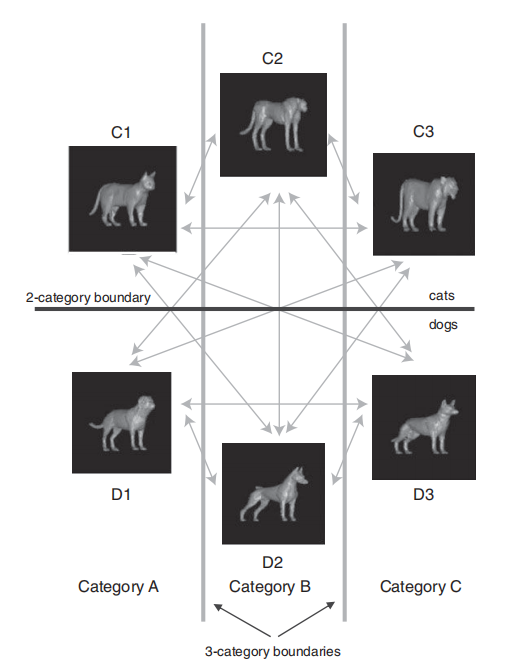
\includegraphics[width=0.6\linewidth]{image_pfc/Fig_7_5}
	\caption{分类任务中使用的刺激。 实验者构建了由不同比例的箭头连接的两种刺激组成的图像。 三只猫特辑 [C1 . . . C3] 和三只狗 [D1 . . . D3] 和它们的变形组合可以归类为狗与猫,由黑色水平线分隔。 或者,可以根据两条灰色垂直线划定的三个类别,对相同的变形刺激进行任意分类。 转载自 Freedman DJ、Riesenhuber M、Poggio T、Miller EK。 2002 年。 视觉分类和灵长类动物前额叶皮层:神经生理学和行为。 神经生理学杂志 88:929–41, © The American Physiological Society, 经许可。}
	\label{fig:fig}
\end{figure}
\par
研究人员继续教猴子新的类别。 这涉及建立新的类别边界,如图 7.4 中的灰色垂直线所示。 然后腹侧 PF 皮层中的细胞编码一个或另一个新类别(图 7.7)。 这一发现的重要性在于腹侧 PF 皮层可以学习的类别的任意性; 它们并不完全取决于共享功能的数量。
\par
扩展这些研究,Cromer 等人。 (2010) 教会了猴子两个独立的类别:猫与狗以及跑车与轿车。 在这种情况下,他们发现了编码这两个类别的多任务细胞。 但是当罗伊等人。 ( 2010 ) 教猴子在猫狗分类的竞争方式之间切换,主要是独立的子种群对这些相互排斥的类别进行编码。 这一结果类似于第 6 章提到的结果,其中背侧 PF皮层中大部分独立的细胞亚群编码当前与先前的空间目标,这也是相互排斥的类别(Genovesio et al. 2006a)。
\par
当然,这些发现并未表明腹侧 PF 皮层细胞对学习至关重要。 下颞叶皮层可以学习类别,而 PF 皮层可以从那里检索信息。 所以弗里德曼等人。 ( 2003 ) 研究了这两个领域的细胞。 下颞叶皮层中的细胞确实编码了一些关于类别的信息,但是,与 PF 皮层中的细胞相比,它们的活动更多地反映了刺激的视觉特征(另见 Meyers et al.2008 年)。 这一发现表明,下颞叶皮层比类别更能代表视觉特征和特征连词,并且分类学习发生在腹侧 PF 皮层。
\par
下颞叶皮层中代表特征结合的细胞(表示为 AB)自动编码具有这两种特征的对象类别,如图 4.3 所示。 因此,例如,仅具有 AB 特征的原型对象将被归类为具有附加特征的对象,例如 ABC、ABCD 等。 同样的原则适用于 PF 皮层内的分类。
\par
因此,类别编码和联合特征编码有着密切的关系,PF皮层和下颞叶皮层的区别不可能像类别和特征编码的区别那么简单。 它们的不同之处在于,PF 皮层从高阶和中阶连词中学习抽象,而下颞叶皮层仅学习中阶连词并且不太灵活。例如,腹侧 PF 皮层似乎在学习具有特征 ABCD 和ABCE 可以属于类别 AB。 但是它的细胞也可以了解到相同的两个对象属于类别 AC。 下颞叶皮层学习中级连接 AB 和 AC 的灵活性似乎较低,主要基于特征而不是分类的附加因素。
\par
鉴于 PF 皮层和下颞叶皮层中的细胞活动都对类别进行编码,我们可能期望在人类受试者对图片进行分类时发现这两个区域的激活。 DeGutis 和 D’Esposito (2009) 教人们根据眼睛的高度和鼻子的长度将面孔分为两类。 在学习这些类别的过程中,中外侧和腹侧 PF 的激活超过了练习类别,并且颞下回的激活仅在主题练习了一个类别。
\begin{figure}
	\centering
	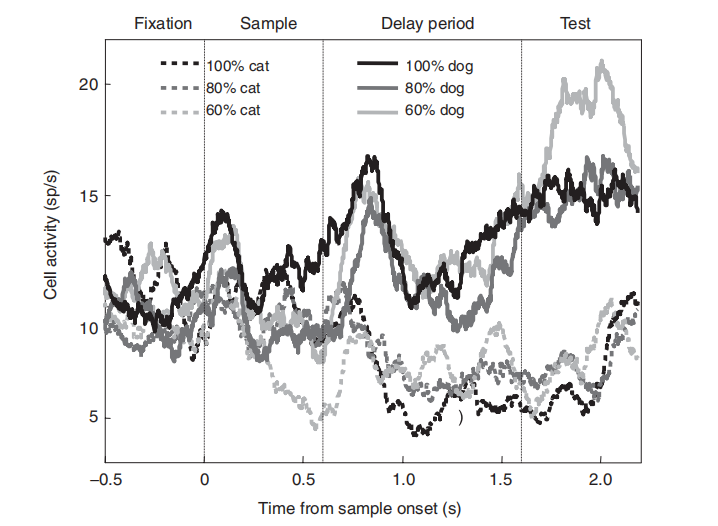
\includegraphics[width=0.6\linewidth]{image_pfc/Fig_7_6}
	\caption{编码“狗”类别的腹侧 PF 皮层细胞。 实线显示细胞在试验中的活动,样本刺激完全(100\%)或主要(60\% 或 80\%)狗画。 虚线表示完全或主要由猫画组成的试验活动。 在延迟期和选择期(测试)期间,与“猫”类别相比,细胞对“狗”类别中的样本具有更高的活性。 转载自 Freedman DJ、Riesenhuber M、Poggio T、Miller EK。 2002 年。 视觉分类和灵长类动物前额皮质:神经生理学和行为。 神经生理学杂志 88:929–41, © The American 生理学会,经许可。}
	\label{fig:fig}
\end{figure}
\par
这些结果可以解释为什么当受试者将图片命名或归类为动物或工具时,激活通常不会发生在 PF 皮质中 (Martin 2007)。 相反,对于多种视觉类别,激活发生在颞叶,对于工具,激活发生在前运动皮层,大概是因为工具可以被处理。 PF 皮质无法显示可检测的激活,因为受试者在早期教育中已经了解了动物和工具的类别。 对于成年人来说,将特定图片分配给一个或另一个类别是自动发生的。
\begin{figure}
	\centering
	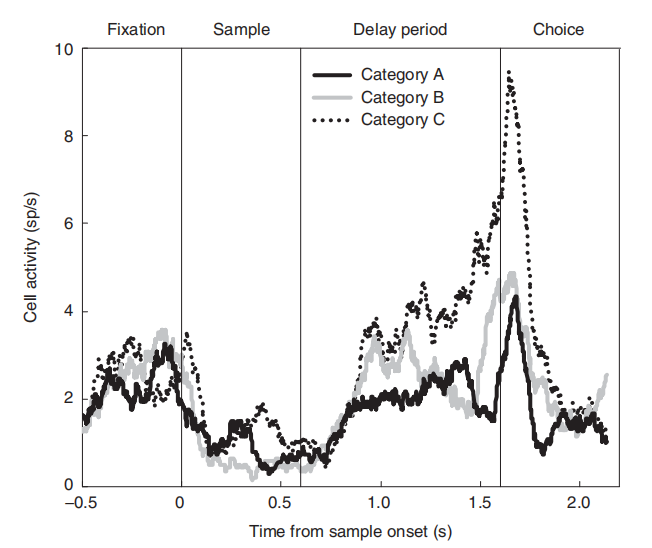
\includegraphics[width=0.6\linewidth]{image_pfc/Fig_7_7}
	\caption{编码任意类别的腹侧 PF 皮层细胞,由图 7.5 中的垂直灰线划分。 该细胞偏好落在最右侧灰色垂直边界右侧的变形刺激,C 类。转载自 Freedman DJ、Riesenhuber M、Poggio T、Miller EK。 视觉分类和灵长类前额叶皮层:神经生理学和行为。 神经生理学杂志 88:929–41,© 2002,美国生理学会,经许可。}
	\label{fig:fig}
\end{figure}
\par
当然,我们并不是说成年人缺乏学习新概念和新范畴的能力。 一个人可以教一只老狗新把戏。 我们将在第 8 章讨论注意力与自动行为的相关主题。就目前的目的而言,可以说对于训练良好的类别,相关的认知操作相对自动地发生,尤其是在成人中。
\par
当图片不属于一个简单的类别时,受试者必须设计新的类别。 在这种情况下,PF 皮层开始参与。 因此,Degutis 和 D’Esposito (2007) 发现,当他们将容易分类的面孔的激活与更难分类的面孔的激活进行比较时,激活仅针对困难的分类任务发生在中外侧和腹侧 PF 中。
\par
我们认为 PF 皮层通过从中阶和高阶联合表示中抽象来学习这些类别。 我们还认为腹侧 PF 皮层可以做到这一点,而下颞叶皮层不能灵活地做到这一点。 和克罗默等人。 ( 2011b ) 表明前运动皮层中的细胞缺乏关于类别的信息,尽管那里的一些细胞活动反映了目标选择。 因此,在不否认其他区域对分类和抽象的贡献的情况下,腹侧 PF 皮层似乎在这些功能中起着关键作用。
\par
Mimaminoto 等。 然而,( 2010 ) 试图证明 PF 皮层甚至对于学习新类别也不是必需的。 他们训练猴子执行一项任务,其中刺激 A 预测一个级别的奖励,而刺激 B 预测另一个级别。 用一点经验,猴子学会归纳; 也就是说,他们将具有刺激 A 某些特征的刺激视为刺激 A。背侧和腹侧 PF 皮层的联合损伤并没有阻止这种泛化。
\par
但是 Mimaminoto 等人使用的任务。 不需要猴子比较项目并在刺激之间构建任意划分,就像弗里德曼等人的实验那样。 Mimaminoto 等人的实验不是学习划分类别的任意细分,而是一种表征真正分类的属性。 仅涉及刺激泛化,也称为特征泛化 (Buckley \& Sigala 2010)。 在刺激泛化中,如果动物已经知道刺激可以预测某事,那么当它看到一个共享其某些特征的刺激时,它也会预测同样的事情:共享的特征越多,预测越强。 这种原始的知觉现象发生在所有脊椎动物身上,与分类无关。
\par
相比之下,弗里德曼等人使用的实验范式。 ( 2002 ) 确实涉及分类。 他们的猴子学会了根据任意划分将变形分为几类,而不是简单地根据一些共享特征。 例如,当他们看到狗的变体时,他们已经学会属于“狗”类别,他们稍后可以学习将相同的变体分类为“猫”。 关键区别涉及对象的学习和任意细分,如 Freedman 等人的实验,而不是 Mimaminoto 等人的实验中的自动刺激泛化。 因此,我们接受基于细胞记录的结论,这表明腹侧 PF 皮层介导了基于学习的视觉对象的灵活分类。
\par
当猴子学会根据它们所属的类别选择对象时,PF 皮层中的细胞活动会对该类别进行编码。 当猴子学习将刺激分类和重新分类到实验者选择施加的任何子集时,细胞会对这些类别进行编码。 尽管有包括腹侧 PF 皮层在内的病变的猴子仍然可以将刺激识别为相似,但它们是通过刺激泛化来识别的,这是一种系统发育上所有脊椎动物共有的古老机制,与真正的分类不同。 当猴子必须通过将任务规则应用于刺激类别(例如身份或匹配规则)来选择目标时,腹侧 PF 皮层发挥最大作用。
\subsection{总结}
\par
当猴子学会根据它们所属的类别选择对象时,PF 皮层中的细胞活动会对该类别进行编码。 当猴子学习将刺激分类和重新分类到实验者选择施加的任何子集时,细胞会对这些类别进行编码。 尽管有包括腹侧 PF 皮层在内的病变的猴子仍然可以将刺激识别为相似,但它们是通过刺激泛化来识别的,这是一种系统发育上所有脊椎动物共有的古老机制,与真正的分类不同。 当猴子必须通过将任务规则应用于刺激类别(例如身份或匹配规则)来选择目标时,腹侧 PF 皮层发挥最大作用。
\section{抽象规则}

\section{改变规则}

\section{抽象策略}

\subsection{结论}


